\chapter{Reciever structure}

\section{Basic receiver structure}


\section{Antenna}
% (beamwidth)

\section{Reciever blocks}
% (Bandwidth, noise figure)

\section{ADC}
% (effective number of bits)


\section{Dynamic range}
Dynamic range in RF systems is the ability of the receiver to pick out weak signals compared to the strong ones(the range of the low signals to the high signals which the receiver can operate). Think about it as trying to hear a person talking when somebody in the room is screaming. For Network analysers the dynamic range is the maximum signal power the receiver can measure minus the noise floor of the receiver. To achieve a higher dynamic range of \gls{VNA} it must be  in tuned-receiver mode (Narrowband). If you reduce the bandwidth then the overall noise floor will go down, so it logical that it would have higher dynamic range. \citep{AgilentNVA} \\
In a normal receiver the dynamic range is set by the sensitivity of the receiver to the Third order intercept point. Third order intercept points are caused by over driving the receiver with too much input and that causes distortion and signal saturation. The sensitivity is more dependent on the operating environment and the receivers noise figure. \citep{understandDynamic} This means that a RF receiver is highly dependent on the mixer and amplifier with regards to dynamic range.\\

\begin{figure}[H]
\centering
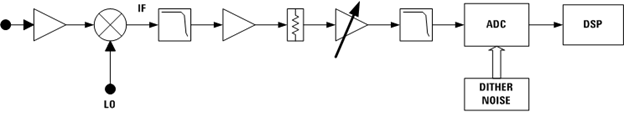
\includegraphics[width=0.90\textwidth]{figures/Block_VNA.png}
\caption{A Typical block diagram of a VNA receiver.}
\label{Block_VNA}
\end{figure}

The setup of the \gls{VNA} measuring would have to take into account some factors to increase the dynamic range and still have the accuracy. Going through the \ref{Block_VNA} in order from left to right.
The \gls{IF} is a frequency that shifted to in order to process the signal easier. This is done in the first stages of a receiver. This frequency is normally lower than the transmitted RF frequency, this especially helps the \gls{ADC} that uses a lower sampling rate. 
By setting the \gls{IF} filter to a very narrow bandwidth (narrowband) the noise floor goes down and increases the dynamic range. The cost of using a narrowband is the measurement time, as the \gls{VNA} would need several sweeps to cover a typical bandwidth. \\

Dynamic range and accuracy are affected by the non-linearity in the receiver chain, the worst part are the mixers,\gls{ADC} and amplifiers since they introduce the most non-linearity. To measure the linearity of a receiver a power change measurements is preformed and compared to a reference level of power change that is accurate. This means that the linearity of a receiver as can be defined as:
\begin{equation}
Linearity = \frac{receiver \\\ measured \\\ power \\\ change}{reference \ power \ change}
\label{Linearity}
\end{equation}
 

Cross talk is the energy leakage between signal paths of the measuring system and it can be a problem in high-loss transmission measurements. This can be fixed by running an isolation calibration \citep{crosstalk}.It occurs below the noise floor so averaging and low \gls{IF} filter bandwidth must be used during calibration.
At low power levels <-70dBm the main non-linearity comes from the \gls{ADC}. Quantizing error occurs when converting from analog to digital signals. The \gls{ADC} used in \gls{VNA} are top of the line and can use a Gaussian noise ditcher to combat the non linear nature of a \gls{ADC}. 

\todo{Add equations to the VNA claims, eg Time used vs Averaging factor(Seeptime vs noise floror reduction)}

In the digital signal processing of the \gls{VNA} averaging be applied to reduce the noise.Given the noise is uncorrelated, by averaging the measured(complex) data the noise component will approach zero.That means that our end signal in the output will be with less noise.Every time that our average is getting doubled, the signal to noise ratio is increased by 3dB. The problem is that by averaging the double of every data point the measurement will take twice as long.\citep{KeysightAVG}. The total noise floor is then given by:

\begin{equation}
Noisefloor = log_{2}(Number \ of \ avrages)\cdot 3dB +10log(B\cdot T_{0}\cdot k)
\label{NFwithAVG}
\end{equation}
 

Equipment drift is another source of error that can occur if we are operating in a place with different environmental factors for a long period of time.

\section{Diversity}
% (effects?)
Diversity is used to combat fading in a wireless system. By using clever techniques you can effectively deliver several copies or replicas of a signal to the receiver. There is a lower chance that all of these copies of signals are going to have a deep fade at the same time \citep[p. 4-6]{diversityFuture}. The overall goal is to provide a gain in signal quality by having several signals that independently fade from each other without the cost of more power consumption, reduced bit rate and complexity or other resources. There are several ways to achieve diversity in a wireless system. \\
Time diversity: By retransmitting the same information you get some diversity gain on the cost of decreased bit/rate. Usually a forward error correction code is added instead of just re transmitting the signals several times. \\
Antenna diversity / Spatial diversity
By having several antennas at both/or the receiver and transmitter a antenna diversity is achieved. With several antennas the signal can be combined together to process the signals into one. To get independently fading signals the signals need to be uncorrelated by separating the antennas least half a wavelength (micro diversity) \citep{diversityAntenna}. Antenna diversity comes at the cost of having to power more than one antenna.



